In this section we evaluate the performance of our optimizations by conducting
experiments on the TPC-H benchmark. 

\subsection{Methodology}

\head{Experimental setup.}
We run all benchmarks under Ubuntu 16.04.6 LTS on a server which has 4 Intel
Xeon E7-4850 2.00GHz (total 40 cores/80 threads) and 128 GB RAM.
We use GCC compiler with the version \textit{v8.1.0} to compile the generated C
code with optimization level \texttt{-O3} and \texttt{-march=native} enabled.
We use the latest MonetDB~\cite{IdreosS2012} released in \textit{Apr2019} with
version v11.33.3, as a baseline comparison for the following HorseIR versions:
(1) HorseIR-noopt: no optimizations;
(2) HorseIR-opt1 : element-wise and pattern-based
fusion from previous work~\OldPaper; and
(3) HorseIR-opt2 : fusion approach presented in this paper.

\head{Execution time.}
Our results present the core execution time of the database query. That is,
compilation time, input data loading time and results output time are not considered
as we want to zoom in on the effects of the optimization. The results present
the average over 15 executions for each query.

% \head{Micro-benchmarks.}

\head{TPC-H SQL benchmarks.}
TPC-H \cite{TPCH2017} is a widely used SQL benchmark suite for analytical data
processing simulating real Business to Consumer (B2C) database applications. The 
database has 8 tables over which 22 queries are defined.  The database size can be
varied by indicating a \textit{scale factor} (SF). For example, a scale factor of 1
(i.e. SF1) means 1GB of input data. With an increasing scale factor, (nearly) each
of the tables holds more data records. Our results are for SF1 but initial results
on larger scale factors show similar results.

%% For this paper, we have selected 8 of the 22 queries (q1/4/6/12/14/16/19/22).
%% These are the queries where the basic built-in functions that we aim to fuse
%% have a major impact on the query execution time. In particular, these queries
%% have a maximum of 2 joins. Joins are very expensive, and in queries with more
%% than 2 joins, the join execution takes up most of the time, thus, the
%% optimizations presented in \OldPaper and in this paper have less impact.
%% Future work will look more closely at fusion potential for join operations.  

For this paper, we have selected the subset of queries in which the basic built-in
functions that we aim to fuse have a major impact on execution time.
In particular, these queries have a maximum of 2 joins. Joins are very
expensive, and in queries with more than 2 joins, the join execution takes up
most of the time, thus, the optimizations presented in \OldPaper and in this
paper have less impact.
Hence, we have such 8 queries (q1/4/6/12/14/16/19/22) in our experiments.
Future work will look more closely at fusion potential for join operations.  

%% In our experiments, we use a number of SFs growing exponentially, i.e.
%% SF1/2/4/8/16, to test the scalability of the generated parallel code.

% \subsection{Micro-benchmarks Results}

\subsection{Execution Time Results}

\begin{figure*}[htbp]
\centering
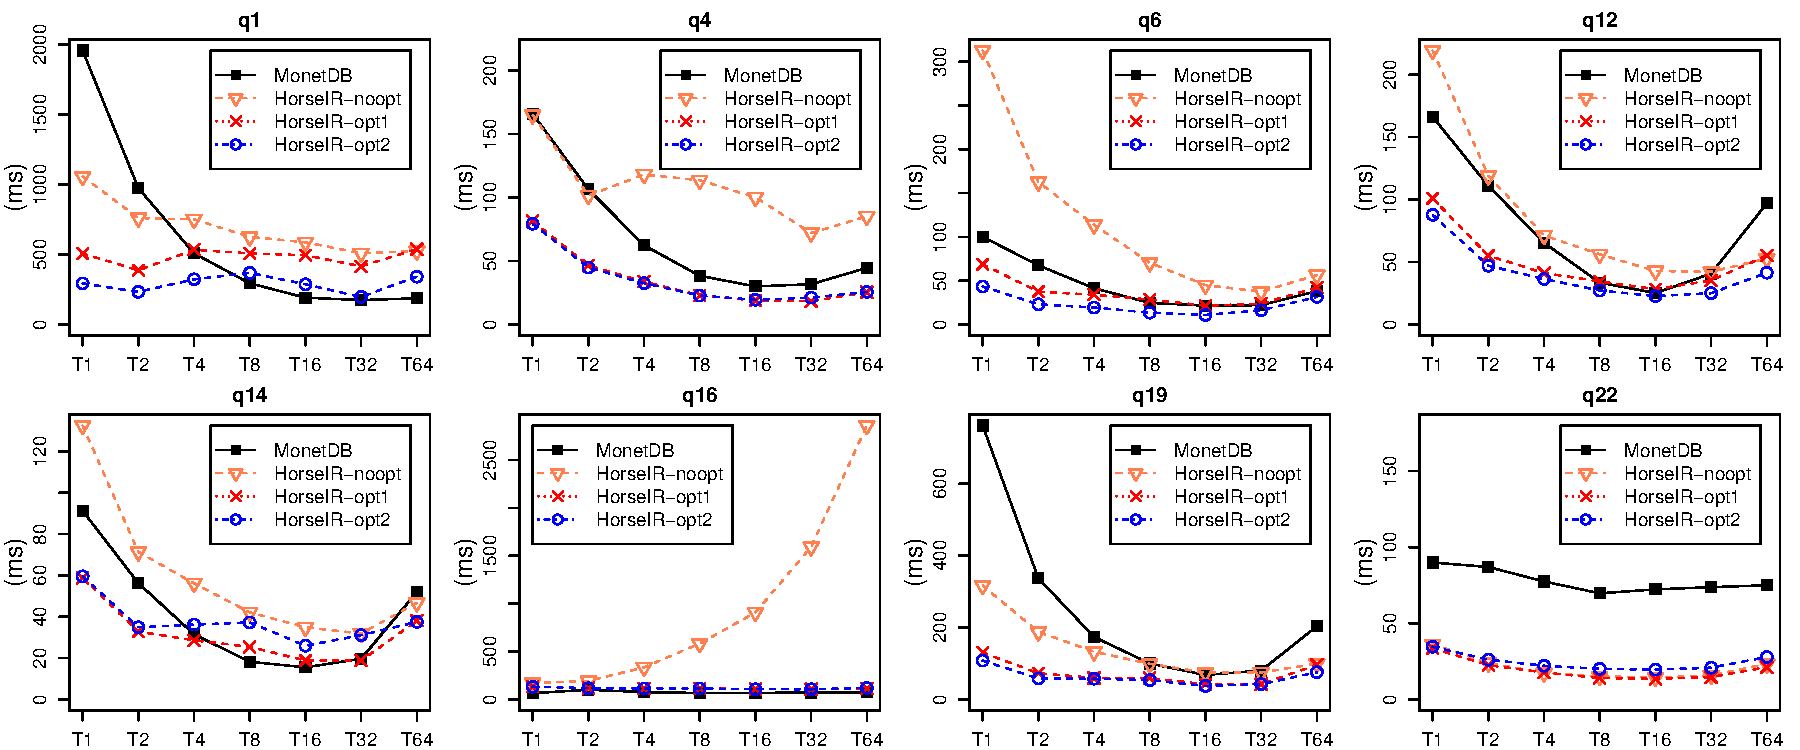
\includegraphics[width=\textwidth]{./src/figure/sf1-v2.pdf}
\caption{The result of TPC-H queries with 1GB input data (SF1).}
\label{fig:tpch_result}
\end{figure*}


\refFig{fig:tpch_result} shows the execution times using MonetDB, HorseIR-noopt,
HorseIR-opt1, and HorseIR-opt2 on SF1 with increasing number of threads. 
Execution time generally decreases with increasing number of threads up to a
certain threshold. The sweet spot for both MonetDB and HorseIR, where the best
performance is achieved, is around 16 threads. Thus, using parallel execution is
beneficial for most queries. In q16, however, there are many small cells (18314 cells,
average size 6.5) and thus our vector parallelization is underutilized.

HorseIR-noopt has the worst performance in most cases showing that optimization
techniques are crucial when trying to exploit array-based languages for query
execution. The two HorseIR-opt versions are generally not as sensitive to the
number of threads as MonetDB, which shows quite bad performance for many
queries when there are only a few threads. 
When looking only at the optimal thread level around 16, MonetDB shows the best
performance for one query, HorseIR-opt1 for one query, HorseIR-opt2 for two
queries, HorseIR-opt1 and HorseIR-opt2 for two queries, and all three behave
very similarly for two queries. That is, there are only 2 queries where our
approach is worse than one of the other approaches, and only by a small margin.

\begin{figure}[htbp]
\centering
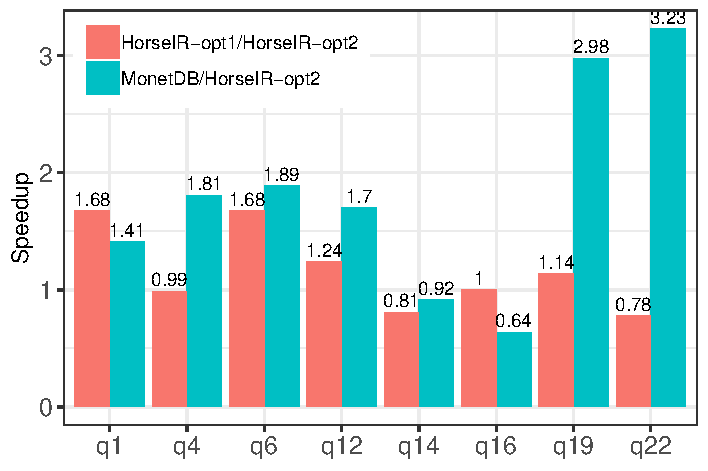
\includegraphics[width=.9\columnwidth]{./src/figure/sf1-speedup.pdf}
\caption{Geometric means of TPC-H queries with 1GB input data (SF1).}
\label{fig:tpch_sf1_speedup}
\end{figure}

To better understand the performance benefit of our approach across all thread counts, 
\refFig{fig:tpch_sf1_speedup} presents the geometric mean speedup for HorseIR-opt2
over HorseIR-opt1 and MonetDB. HorseIR-opt2 provides an improvement over
MonetDB (speedup > 1) for all but one query and the improvement is quite significant. 

\textit{When we are better.}
In q1, our optimizer identifies eight fusible sections that are merged into one
big loop. In q6, two blocks of element-wise functions separated by a non-element-wise
statement (\texttt{@compress}) are fused together. In both cases, intermediate
results are avoided and performance improved. In q12/q19, more statements
are fused and less intermediate results created but the effect is weaker.

\textit{When we are worse.}
In q14/q22, the fused loop sizes are relatively small with long expressions in
the body. Thus, fusion introduces complexity without significantly fewer
iterations. 

\textit{When we behave similarly.}
For queries q4 and q16, the filters are very selective and only a few rows
qualify. Thus, fusing loops has little benefit but also does not harm the
execution.

\new{
Compared to HorseIR-opt1, we improve four queries, are the same for two
queries, and are worse for two queries giving a geometric speedup of 12\%. This
performance improvement is due to the significant increase in fused statements
discussed in \refSec{fusing_stmts}. Our technique thus effectively identifies
fusion opportunities in HorseIR programs generated from SQL queries using a
more systematic and general approach than patterns.}

%%% The main computation part of the queries have operators unable to be fused.
%%% That means we can either improve the operators with efficient implementations
%%% or come up with a new group and a new analysis in order to achieve code fusion.


%%% \todo{The results of q1 and q14 are much slower than MonetDB, however, they are
%%% faster than MonetDB on the previous paper.  (Already send email to Andrew to ask
%%% for his help, maybe a RAM failure again)}

%%% \todo{Add scalability}

\subsection{Fusing Statements} \label{fusing_stmts}

\begin{figure}[htbp]
\centering
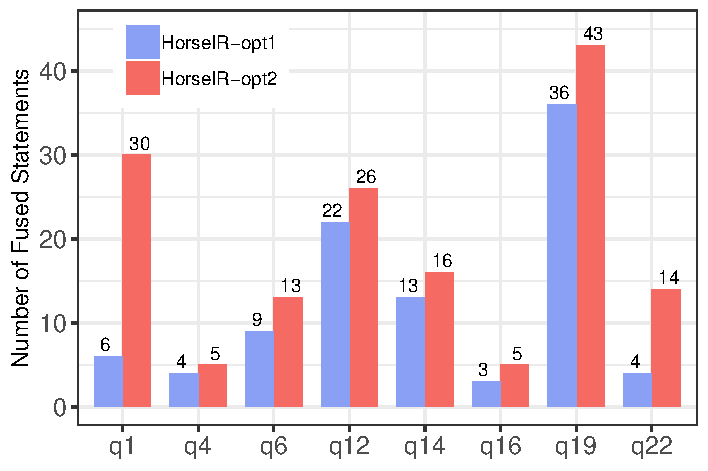
\includegraphics[width=.9\columnwidth]{./src/figure/bar-number.pdf}
\caption{Number of element-wise fused statements in HorseIR-opt1 and our new
fusion in HorseIR-opt2.}
\label{fig:opt_number}
\end{figure}

\refFig{fig:opt_number} shows the the number of fused statements using
element-wise fusion in HorseIR-opt1 and the more general function fusion in
HorseIR-opt2. Pattern-based fusion is not shown as both approaches use the
same patterns. 

We can see that our approach always fuses more statements than HorseIR-opt1.
In q1 and q22, the large increase in fused statements is due to list-related
statements that can now be fused without fixed patterns. Furthermore, our optimizer
exploits fusion of mixed function kinds such as element-wise and reduction functions.
However, as seen in the previous analysis, fusing is not always beneficial. In q22,
we fuse significantly more than HorseIR-opt1, but the loops now contain complex
expressions which result in worse performance compared to HorseIR-opt1.

\begin{figure}[htbp]
\centering
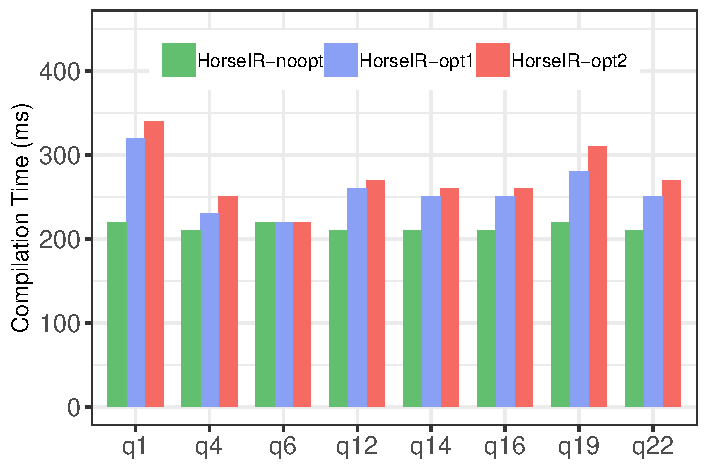
\includegraphics[width=.9\columnwidth]{./src/figure/compile-time.pdf}
\caption{Compilation time for generated C code.}
\label{fig:compilation_time}
\end{figure}

\new{The compilation time of the generated C code seen in \refFig{fig:compilation_time}
shows that our technique is slower to generate the binary than more naive approaches.
However, the increase in compilation time is associated with exploitation of additional
optimization opportunities that benefit the execution time. With large data sizes
common to modern applications or repeated query execution, the compilation time can
be effectively amortized.}

%%% In the query q1, the number of patterns are significantly reduced because a set
%%% of fusion nodes can be further merged into a single loop due to the same loop
%%% structure.  In q6, the pattern for common masks are removed because the result
%%% of boolean selection will be reduced into a single number so that their the
%%% intermediate results should be discard.


%%% \begin{table}[htbp]
%%% \centering
%%% \caption{Number of statements fused in benchmark queries under two versions of optimizations}
%%% \label{table:opt_number}
%%% \begin{tabular}{|c||c|c|c|c|}
%%% \hline
%%% & \multicolumn{2}{c||}{HorseIR-opt1} & \multicolumn{2}{c|}{HorseIR-opt2} \\ \hline
%%% Query & Patterns & Elementwise & Patterns & Fusion \\ \hline
%%% \hline
%%% q1  & 11 & 2 & 3 & 1 \\ \hline
%%% q4  & 3 & 1 & 2 & 2 \\ \hline
%%% q6  & 1 & 1 & 0 & 1 \\ \hline
%%% q12 & 3 & 5 & 3 & 3 \\ \hline
%%% q14 & 2 & 4 & 2 & 4 \\ \hline
%%% q16 & 5 & 1 & 5 & 2 \\ \hline
%%% q19 & 2 & 6 & 1 & 6 \\ \hline
%%% q22 & 4 & 2 & 2 & 3 \\ \hline
%%% \end{tabular}
%%% \end{table}


\subsection{Discussion}

In summary, we can see that fusion across statements is beneficial in many
cases. However, we can see two situations where one has to be more careful about
applying fusion. The first is that fusing too many statements might become
sub-optimal. We believe this is due to the increased pressure on register
allocation. Maybe one could create heuristics to determine a maximum number of
statements to be fused. 

The second situation arises when filtering conditions have a high selectivity,
e.g., when only 10 out of a million records qualify. Then the benefit of
avoiding intermediate results is negligible, while the overhead of code fusion
might become a factor. 
If one had enough information about the properties of the actual data, such
unnecessary fusions could be avoided. Therefore, introducing runtime optimizations
to decide when to fuse is an interesting avenue for future research.